% Szglab4
% ===========================================================================
%
\chapter{Analízis modell kidolgozása 1}

\thispagestyle{fancy}

\section{Objektum katalógus}

\subsection{\bf Parser}
Áramkör értelmező objektum, feladata, hogy a paraméterként átadott, illetve fájlban elhelyezett komponenseket értelmezze, a kapcsolatokat feltérképezze, elvégezze az összeköttetéseket, és ezáltal felépítse az áramkört.

\subsection{\bf ConsoleView}
Az áramkör karakteres megjelenítéséért, és a szimuláció során a változások megjelenítésének frissítéséért felelős objektum.

\subsection{\bf Simulation}
Szimuláció objektum. A szimulációért felelős. Elindítja a jelgenerátor léptetőt, s utasítja az áramkört a kiértékelésre, és figyeli ha az áramkörben változás történt. Ha változás megadott lépésen belül nem történt, tájékoztatja a felhasználót, hogy nincs stacionárius állapot. Továbbá a megadott grafikai megjelenítőt frissíti.

\subsection{\bf Circuit}
Az áramkör objektum. Ezen objektum feladata a jelgenerátor léptető kérésére a jelgenerátorok léptetése, az áramkörben található komponensek utasítása arra, hogy töröljék a "már kiértékelve" flaget, hogy ezáltal a következő kiértékelés kezdeményezésre továbbítsák azt bemeneteik számára is.
Továbbá feladata a kiértékelés elindítása az összes kijelzőre, mert a rendszer kiértékelése a kijelzők kiértékelésével kezdődik.


\subsection{\bf SequenceGeneratorStepper}
Jelgenerátor léptető objektum. Feladata, hogy a szimulációt utasítsa, hogy az áramkörben megtalálható jelgenerátorokat léptesse.

\subsection{\bf SequenceGenerator}
Jelgenerátor, az áramkört felépítő egyik alapelem, kiértékelési kezdeményezés hatására az előre betáplált jelsorozatot soron következő elemét állítja be aktuális értékként, így azon komponensek melyek bemenetére a Jelgenerátor van kötve, elérik aktuális értékét. Bemenete nem komponens jellegű így nem kezel más komponenseket.

\subsection{\bf AndGate}
ÉS kapu, az áramkör egyik alapeleme. Bemeneteire kötött komponensek kiértékelését kezdeményezi, s a kapott értékek logikai ÉS kapcsolatát valósítja meg, ezáltal a kimenetére kötött komponens eléri az aktuális értékét.Figyeli hogy ha már kiértékelődött akkor nem kezdeményezi a bemenetére kötött komponensek kiértékelését.

\subsection{\bf OrGate}
VAGY kapu, az áramkör egyik alapeleme. Bemeneteire kötött komponensek kiértékelését kezdeményezi, s a kapott értékek logikai VAGY kapcsolatát valósítja meg, ezáltal a kimenetére kötött komponens eléri az aktuális értékét.Figyeli hogy ha már kiértékelődött akkor nem kezdeményezi a bemenetére kötött komponensek kiértékelését.

\subsection{\bf Inverter}
Invertáló, az áramkör alapelemei közé tartozik. A bemenetére érkező jel logikai negáltját valósítja meg, így a kimenetén levő komponens eléri aktuális értékét.

\subsection{\bf Gnd}
Föld, az áramkört felépítő egyik elem, aktuális értéke minden kiértékelési kérésre logikai hamis. Bemenete nem létezik, így nem kezdeményez további kiértékeléseket. Állandó értéke logikai hamis.

\subsection{\bf Vcc}
Áramkör alapeleme, mely kiértékelési kezdeményezésre aktuális értékét logikai igaz ra állítja be. Állandó értéke logikai igaz.

\subsection{\bf Led}
Egy kijelző az áramkör alapeleme, bemenetére kötött komponens kiértékelését kezdeményezi, és ezáltal az aktuális értékét egy a felhasználó számára érzékelhető módon kijelzi.

\subsection{\bf Toggle}
Kapcsoló, az áramkört felépítő elem, felhasználói interakciót követően, az aktuális értékét lehet állítani. Komponens bemenete nincs, így nem kezel további komponenseket.

\section{Osztályok leírása}
\comment{Az előző alfejezetben tárgyalt objektumok felelősségének formalizálása attribútumokká, metódusokká. Csak publikus metódusok szerepelhetnek. Ebben az alfejezetben megjelennek az interfészek, az öröklés, az absztrakt osztályok. Segédosztályokra még mindig nincs szükség. Az osztályok ABC sorrendben kövessék egymást. Interfészek esetén az Interfészek, Attribútumok pontok kimaradnak.}

\subsection{Circuit}
\begin{itemize}
\item Felelősség\\
Feladata a jelgenerátor léptető kérésére a jelgenerátorok léptetése, a feldolgozó  által létrehozott komponensek felvétele az áramkörbe, illetve ezek utasítása arra,  hogy töröljék a "már kiértékelve" flaget egy adott kiértékelési ciklus előtt, hogy ezáltal a  ciklusban minden kimenet értéke frissülhessen.  Továbbá feladata a kiértékelés elindítása az összes kijelzőre, mert a rendszer kiértékelése  a kijelzők kiértékelésével kezdődik.
\item Ősosztályok:\ Object $\rightarrow{}$ Circuit.
\item Interfészek: (nincs)
\item Attribútumok $\ $
\begin{itemize}
	\item \texttt{private HashMap componentMap} Komponenseket tartalmazó HashMap
	\item \texttt{private List displays} Megjelenítő típusú komponensek
	\item \texttt{private Simulation simulation} Áramkört éppen szimuláló objektum
	\item \texttt{private List sources} Jelforrás típusú komponensek
	\item \texttt{private boolean stable} Áramkör stabilitása
\end{itemize}
\item Metódusok$\ $
\begin{itemize}
	\item \texttt{public AbstractComponent addComponent(AbstractComponent component)}: Komponens hozzáadása az áramkörhöz.
	\item \texttt{public void doEvaluationCycle()}: Egy kiértékelési ciklus lefuttatása. Az áramkörtől ezután lekérdezhető, hogy  stabil (nem változott semelyik komponens kimenete az utolsó futtatás óta)  vagy instabil állapotban van-e.
	\item \texttt{public AbstractComponent getComponentByName(String name)}: Lekérünk egy komponenst az áramkörtől a neve alapján.
	\item \texttt{public List getDisplays()}: Megjelenítő típusú komponeseket adja vissza.
	\item \texttt{public List getSources()}: Jelforrás típusú komponenseket adja vissza.
	\item \texttt{public boolean isStable()}: Áramkör stacionárius állapotának lekérdezése.
	\item \texttt{public int loadSources(String fileName)}: Fájlból betölti a jelforrások állapotát.
	\item \texttt{public int saveSources(String fileName)}: Elmenti fájlba a jelforrások állapotát.
	\item \texttt{public void setSimulation(Simulation simulation)}: Szimuláció beállítása. Ez a szimuláció létrejöttekor hívódik meg.
	\item \texttt{public void setStable(boolean stable)}: Áramkör stabilitásának beállítása.
	\item \texttt{public void simulationShouldBeWorking()}: Jelzi a szimuláció felé, hogy új ciklust kell indítani. Ezt egy jelforrás  beállítása után hívjuk meg.
	\item \texttt{public void stepGenerators()}: Jelgenerátorok a szimuláció szemszögéből nézve, egyszerre történő  léptetése.
\end{itemize}
\end{itemize}

\subsection{SequenceGeneratorStepper}
\begin{itemize}
\item Felelősség\\
Jelgenerátor-léptető szál. Feladata, hogy az áramkört utasítsa a jelgenerátorok léptesésére  a felhasználó által konfigurálható időközönként.
\item Ősosztályok:\ Object $\rightarrow{}$ Thread $\rightarrow{}$ SequenceGeneratorStepper.
\item Interfészek: (nincs)
\item Attribútumok $\ $
\begin{itemize}
	\item \texttt{private long pause} Szünet két léptetés között -- felhasználó által konfigurálható
	\item \texttt{private boolean shouldRun} A futási ciklus változója; ha ez hamis lesz, akkor leáll a szál
	\item \texttt{private Simulation simulation} A szimuláció, aki számára lépteti a jelgenerátorokat
\end{itemize}
\item Metódusok$\ $
\begin{itemize}
	\item \texttt{public void run()}: Megadott időközönként az áramkörön meghívjuk a stepGenerators() metódust.
	\item \texttt{public void setPause(long pause)}: Két léptetés között eltelt idő állítása (léptetési sebesség)
\end{itemize}
\end{itemize}

\subsection{Simulation}
\begin{itemize}
\item Felelősség\\
Egy szimulációt reprezentáló objektum.  Futásakor elindítja a jelgenerátor léptetőt, s utasítja az áramkört több kiértékelési  ciklus lefuttatásához, amíg az áramkörben van változás. Ha a változás megadott lépésen belül  nem áll meg, tájékoztatja a felhasználót, hogy nincs stacionárius állapot.  Amikor leállítódik, a jelgenerátor-léptetőt is leállítja.  A szál természetéből adódóan többet nem indítható el, új szimulációhoz új példányt kell létrehozni.
\item Ősosztályok:\ Object $\rightarrow{}$ Thread $\rightarrow{}$ Simulation.
\item Interfészek: (nincs)
\item Attribútumok $\ $
\begin{itemize}
	\item \texttt{private Circuit circuit} Szimulált áramkör
	\item \texttt{private int counter} ciklusszámláló, amely ha eléri a \textit{cycleLimit}-et, akkor leáll a szimuláció és jelezzük a felhasználónak.
	\item \texttt{private State currentState} Szimuláció jelenlegi állapota
	\item \texttt{private static final int cycleLimit} cikluslimit
	\item \texttt{private final Object lock} segéd lock objektum
	\item \texttt{private SequenceGeneratorStepper seqGenStepper} Jelgenerátor-léptető, amit elindítunk, ha elindul a szimuláció.
	\item \texttt{private boolean shouldRun} A futási ciklus változója; ha ez hamis lesz, akkor leáll a szál
	\item \texttt{private final Object synchObj} segéd sync objektum, ami a szál altatásához kell.
\end{itemize}
\item Metódusok$\ $
\begin{itemize}
	\item \texttt{public Circuit getCircuit()}: Szimulált áramkör lekérdezése
	\item \texttt{public Object getLock()}: Egy lock objektum, a szálak egymást kizáráshoz kell.
	\item \texttt{public void run()}: A szál futása közben történő dolgokat valósítjuk meg. Lásd \ref{fig:sim_running1} és \ref{fig:sim_running2} ábra.
	\item \texttt{public void setState(State state)}: Állapot beállítása.
\end{itemize}
\end{itemize}

\subsection{Simulation.State}
\begin{itemize}
\item Felelősség\\
Szimuláció állapotait írja le
\item Ősosztályok:\ Object $\rightarrow{}$ Enum $\rightarrow{}$ Simulation.State.
\item Interfészek: (nincs)
\item Attribútumok $\ $
\begin{itemize}
	\item \texttt{public static final State PAUSED} Szimuláció szüneteltetve van, a következő jelforrás változásig.
	\item \texttt{public static final State STOPPED} Szimuláció leállt, ahhoz, hogy bármi történjen az áramkörre újra kell indítani.
	\item \texttt{public static final State WORKING} Szimuláció éppen dolgozik, egy konkrét jelforrás-kombinációt alkalmazva dolgoztatja az áramkört
\end{itemize}
\item Metódusok$\ $
\begin{itemize}
	\item \texttt{public static State valueOf(String name)}: 
 % TODO
	\item \texttt{public static State[] values()}: 
 % TODO
\end{itemize}
\end{itemize}

\subsection{Value}
\begin{itemize}
\item Felelősség\\
Az áramkörben előfordulható értéket reprezentál.
\item Ősosztályok:\ Object $\rightarrow{}$ Enum $\rightarrow{}$ Value.
\item Interfészek: (nincs)
\item Attribútumok $\ $
\begin{itemize}
	\item \texttt{public static final Value FALSE} 
 % TODO
	\item \texttt{public static final Value TRUE} 
 % TODO
\end{itemize}
\item Metódusok$\ $
\begin{itemize}
	\item \texttt{public Value invert()}: Invertálja az adott értéket. Ennek addig van értelme, amíg 2 féle  állapot fordulhat elő a rendszerben.
	\item \texttt{public static Value valueOf(String name)}: 
 % TODO
	\item \texttt{public static Value[] values()}: 
 % TODO
\end{itemize}
\end{itemize}


\subsection{AbstractComponent}
Absztrakt osztály.
\begin{itemize}
\item Felelősség\\
Egy komponens absztrakt megvalósítása, ebből származik az összes többi  komponens. A közös logikát valósítja meg. A gyakran használt dolgokra  ad alapértelmezett implementációt (összekötés, bemenetek kiértékelése stb.)
\item Ősosztályok: (nincs)
\item Interfészek: (nincs)
\item Attribútumok $\ $
\begin{itemize}
	\item \texttt{protected String name}: Komponens neve (ahogy az áramkörben azonosítjuk)
	\item \texttt{private boolean changed}: Azt mutatja meg, hogy változott-e valamelyik kimenete a komponensnek. Ez a flag az \texttt{evaluate()} meghívásánál számolódik ki, vagyis azt jelzi, hogy két kiértékelés között változott-e a kimenet.
	\item \texttt{protected boolean alreadyEvaluated}: "Kiértékelt" flag, ha ez be van billenve, akkor nem számolunk újra, csak visszaadjuk az előzőleg kiszámolt értéket.
	\item \texttt{protected Value[] values}: Kimeneteken lévő értékek. Ez frissül az \texttt{evaluate()} meghívására, ha még nem volt kiértékelve.
	\item \texttt{protected AbstractComponent[] inputs}: A bemenetekre kötött komponensek.
	\item \texttt{protected int[] indices}: Itt tároljuk, hogy melyik bemenetre, az adott komponens melyik kimenetét kötöttük.
\end{itemize}
\item Metódusok$\ $
\begin{itemize}
	\item \texttt{String getName()}: Név lekérdezése
	\item \texttt{void setName(String name)}: Név beállítása (változó, amivel azonosítjuk)
	\item \texttt{addTo(Circuit c)}: Meghívja az áramkör \texttt{add(AbstractComponent ac)} metódusát.
	\item \texttt{Value[] evaluate()}: Komponens kimenetein lévő értékek újraszámolása (ha a kiértékelt flag, nincs beállítva) a bemenetek alapján. A kimeneteken lévő értékekkel tér vissza.
	\item \texttt{void clearEvaluatedFlag()}: Töröljük a komponens "kiértékelt" flagjét.
	\item \texttt{getValue(int idx)}: Visszaadja a paraméterben megadott indexű kimenet értékét.
	\item \texttt{boolean isChanged()}: Changed flag lekérdező metódusa.
	\item \texttt{void setInput(int inputPin, AbstractComponent component, int outputPin)}: Beállítunk egy bemenetet (adott bemeneti lábra rákötjük az adott komponens adott kimeneti lábát).
	\item \texttt{void setInputPinsCount()}: \comment{KELL EZ? (impl.ben igen, de most a rajzon nem szerepel}
\end{itemize}
\end{itemize}

\subsection{FlipFlop}
Absztrakt osztály.
\begin{itemize}
\item Felelősség\\
Flipflopok ősosztálya, itt vannak leírva a flipflopok közös logikája.
\item Ősosztályok:\ AbstractComponent
\item Interfészek: (nincs)
\item Attribútumok $\ $
\begin{itemize}
	\item \texttt{protected Value q}: A flip-flopban tárolt érték (az előző állapot)
	\item \texttt{protected Value clk}: A rendszer előző stabil állapotánál mért flip-flop órajel-bemenetére érkező érték (ennek segítségével tudunk detektálni élváltozást).
\end{itemize}
\item Metódusok$\ $
\begin{itemize}
	\item \texttt{addTo(Circuit c)}: Meghívja az áramkör \texttt{add(FlipFlop ff)} metódusát.
	\item \texttt{void commit()}: Az FF jelenlegi kimenetét és az órajel bemenetét elmentjük a \texttt{q} és \texttt{clk} attribútumba. Ezt akkor kell meghívni, amikor az áramkör az adott áramköri bemenetekre stabil állapotba ért.
	\item \texttt{boolean isActive()}: Számolhat-e az FF? Ezt kell ellenőrizniük a konkrét flipflop implementációknak, hiszen ekkor kellhet a belső állapottól eltérő állapotot kiadni.
\end{itemize}
\end{itemize}

\subsection{DisplayComponent}
Absztrakt osztály.
\begin{itemize}
\item Felelősség\\
Megjelenítő típusú komponensek ősosztálya.
\item Ősosztályok:\ AbstractComponent.
\item Interfészek: (nincs).
\item Attribútumok $\ $
\begin{itemize}
	\item (nincs)
\end{itemize}
\item Metódusok$\ $
\begin{itemize}
\item \texttt{addTo(Circuit c)}: Meghívja az áramkör \texttt{add(DisplayComponent dc)} metódusát (és az ősosztály implementációját is -- hiszen ugyanúgy kell regisztrálni a megjelenítőket is, mint a többi komponenst).
\end{itemize}
\end{itemize}

\subsection{SourceComponent}
Absztrakt osztály.
\begin{itemize}
\item Felelősség\\
Jelforrás típusú komponensek ősosztálya.
\item Ősosztályok:\ AbstractComponent.
\item Interfészek: (nincs).
\item Attribútumok $\ $
\begin{itemize}
	\item (nincs)
\end{itemize}
\item Metódusok$\ $
\begin{itemize}
\item \texttt{addTo(Circuit c)}: Meghívja az áramkör \texttt{add(SourceComponent dc)} metódusát (és az ősosztály implementációját is -- hiszen ugyanúgy kell regisztrálni a jelforrásokat is, mint a többi komponenst).
	\item \texttt{abstract Value[] getValues()}: Lekérhetjük a jelforrás értékeit. Ennek megvalósítása a konkrét implementációk feladata.
	\item \texttt{abstract setValues(Value[] values)}: Beállítjuk a jelforrás értékét. Ennek megvalósítása a konkrét implementációk feladata. (pl. kapcsoló csak 1 elemű tömböt kaphat)
\end{itemize}
\end{itemize}


\subsection{AndGate}
\begin{itemize}
\item Felelősség\\
ÉS kapu, az áramkör egyik alapeleme. Bemeneteire kötött komponensek  kiértékelését kezdeményezi, s a kapott értékek logikai ÉS kapcsolatát  valósítja meg, amit a kimenetén kiad.
\item Ősosztályok:\ Object $\rightarrow{}$ AbstractComponent $\rightarrow{}$ AndGate.
\item Interfészek: (nincs)
\item Attribútumok $\ $
\begin{itemize}
\item (nincs)
\end{itemize}
\item Metódusok$\ $
\begin{itemize}
\item (nincs)
\end{itemize}
\end{itemize}

\subsection{FlipFlopD}
\begin{itemize}
\item Felelősség\\
D flipflop, mely felfutó órajelnél beírja a belső memóriába az adatbemeneten (D)  lévő értéket.
\item Ősosztályok:\ Object $\rightarrow{}$ AbstractComponent $\rightarrow{}$ FlipFlop $\rightarrow{}$ FlipFlopD.
\item Interfészek: (nincs)
\item Attribútumok $\ $
\begin{itemize}
\item (nincs)
\end{itemize}
\item Metódusok$\ $
\begin{itemize}
\item (nincs)
\end{itemize}
\end{itemize}

\subsection{FlipFlopJK}
\begin{itemize}
\item Felelősség\\
JK flipflop, mely a belső memóriáját a Követelmények résznél leírt módon  a J és K bemenetektől függően változtatja.
\item Ősosztályok:\ Object $\rightarrow{}$ AbstractComponent $\rightarrow{}$ FlipFlop $\rightarrow{}$ FlipFlopJK.
\item Interfészek: (nincs)
\item Attribútumok $\ $
\begin{itemize}
\item (nincs)
\end{itemize}
\item Metódusok$\ $
\begin{itemize}
\item (nincs)
\end{itemize}
\end{itemize}

\subsection{Gnd}
\begin{itemize}
\item Felelősség\\
A "föld" komponens, mely állandóan a hamis értéket adja ki. Nincs bemenete.
\item Ősosztályok:\ Object $\rightarrow{}$ AbstractComponent $\rightarrow{}$ Gnd.
\item Interfészek: (nincs)
\item Attribútumok $\ $
\begin{itemize}
\item (nincs)
\end{itemize}
\item Metódusok$\ $
\begin{itemize}
\item (nincs)
\end{itemize}
\end{itemize}

\subsection{Inverter}
\begin{itemize}
\item Felelősség\\
Inverter alkatrész, mely invertálva adja ki a kimenetén a bemenetén  érkező jelet.
\item Ősosztályok:\ Object $\rightarrow{}$ AbstractComponent $\rightarrow{}$ Inverter.
\item Interfészek: (nincs)
\item Attribútumok $\ $
\begin{itemize}
\item (nincs)
\end{itemize}
\item Metódusok$\ $
\begin{itemize}
\item (nincs)
\end{itemize}
\end{itemize}

\subsection{Led}
\begin{itemize}
\item Felelősség\\
Egy LED-et reprezentál, mely világít, ha bemenetén igaz érték van.  3 féle színe lehet, ezeket a Color enumeráció határozza meg.
\item Ősosztályok:\ Object $\rightarrow{}$ AbstractComponent $\rightarrow{}$ Led.
\item Interfészek: IsDisplay.
\item Attribútumok $\ $
\begin{itemize}
\item (nincs)
\end{itemize}
\item Metódusok$\ $
\begin{itemize}
\item (nincs)
\end{itemize}
\end{itemize}

\subsection{Mpx}
\begin{itemize}
\item Felelősség\\
4-1-es multiplexer, melynek a bemeneti lábak sorrendje a következő:  D0, D1, D2, D3, S0, S1. Ahol Dx az adatbemenetek, Sy a kiválasztóbemenetek.  Kimenetén a kiválasztóbemenetektől függően valamelyik adatbemenet kerül kiadásra.
\item Ősosztályok:\ Object $\rightarrow{}$ AbstractComponent $\rightarrow{}$ Mpx.
\item Interfészek: (nincs)
\item Attribútumok $\ $
\begin{itemize}
\item (nincs)
\end{itemize}
\item Metódusok$\ $
\begin{itemize}
\item (nincs)
\end{itemize}
\end{itemize}

\subsection{OrGate}
\begin{itemize}
\item Felelősség\\
VAGY kapu, az áramkör egyik alapeleme. Bemeneteire kötött komponensek  kiértékelését kezdeményezi, s a kapott értékek logikai VAGY kapcsolatát  valósítja meg, amit a kimenetén kiad.
\item Ősosztályok:\ Object $\rightarrow{}$ AbstractComponent $\rightarrow{}$ OrGate.
\item Interfészek: (nincs)
\item Attribútumok $\ $
\begin{itemize}
\item (nincs)
\end{itemize}
\item Metódusok$\ $
\begin{itemize}
\item (nincs)
\end{itemize}
\end{itemize}

\subsection{SequenceGenerator}
\begin{itemize}
\item Felelősség\\
Jelgenerátort reprezentál, amely a beállított bitsorozatot adja ki. A  SequenceGeneratorStepper feladata, hogy a step() metódust meghívja ezen osztály  példányain. Azokat a FF-eket vezérli, melyek CLK bemenetére ez a komponens van kötve,  vagyis ha éppen felfutó él jön, akkor ezeket engedélyezi különben nem.
\item Ősosztályok:\ Object $\rightarrow{}$ AbstractComponent $\rightarrow{}$ SequenceGenerator.
\item Interfészek: IsSource.
\item Attribútumok $\ $
\begin{itemize}
	\item \texttt{private List ffList}: Azon FF-ek listája, melyekre ez a jelgenerátor van bekötve a CLK bemenetre.
	\item \texttt{private int index}: Bitsorozat egy indexe, ez határozza meg, hogy éppen melyik értéket adja ki.
	\item \texttt{private Value[] sequence}: Tárolt bitsorozat
\end{itemize}
\item Metódusok$\ $
\begin{itemize}
	\item \texttt{void addFlipFlop(FlipFlop ff)}: A flipflop-ot feliratkoztatjuk a jelgenerátorhoz, így ha felfutó él lesz,  akkor tudunk neki jelezni.
	\item \texttt{Value[] getValues()}: Jelgenerátor bitsorozatának lekérdezése
	\item \texttt{void setValues(Value[] values)}: Jelgenerátor bitsorozatának beállítása
	\item \texttt{void step()}: A jelgenerátor lép, a bitsorozat következő elemére ugrik. A következő léptetésig  ez kerül kiadásra a kimeneteken.
\end{itemize}
\end{itemize}

\subsection{SevenSegmentDisplay}
\begin{itemize}
\item Felelősség\\
7-szegmenses kijelzőt reprezentál, melynek 7 bemenete vezérli a  megfelelő szegmenseket, ezek világítanak, ha az adott bemenetre logikai  igaz van kötve.
\item Ősosztályok:\ Object $\rightarrow{}$ AbstractComponent $\rightarrow{}$ SevenSegmentDisplay.
\item Interfészek: IsDisplay.
\item Attribútumok $\ $
\begin{itemize}
\item (nincs)
\end{itemize}
\item Metódusok$\ $
\begin{itemize}
\item (nincs)
\end{itemize}
\end{itemize}

\subsection{Toggle}
\begin{itemize}
\item Felelősség\\
Kapcsoló jelforrás, melyet a felhasználó szimuláció közben kapcsolgathat.
\item Ősosztályok:\ Object $\rightarrow{}$ AbstractComponent $\rightarrow{}$ Toggle.
\item Interfészek: IsSource.
\item Attribútumok $\ $
\begin{itemize}
\item (nincs)
\end{itemize}
\item Metódusok$\ $
\begin{itemize}
	\item \texttt{Value[] getValues()}: Lekérjük a kapcsoló értékét (1 elemű tömb)
	\item \texttt{void setValues(Value[] values)}: Kapcsoló állapotának változtatása, csak 1 elemű tömböt kaphat paraméterül.
\end{itemize}
\end{itemize}

\subsection{Vcc}
\begin{itemize}
\item Felelősség\\
A tápfeszültés komponens, ami konstans igaz értéket ad. Nincs bemenete.
\item Ősosztályok:\ Object $\rightarrow{}$ AbstractComponent $\rightarrow{}$ Vcc.
\item Interfészek: (nincs)
\item Attribútumok $\ $
\begin{itemize}
\item (nincs)
\end{itemize}
\item Metódusok$\ $
\begin{itemize}
\item (nincs)
\end{itemize}
\end{itemize}


\subsection{Controller}
Interfész.
\begin{itemize}
\item Felelősség\\

 % TODO
\item Ősosztályok\ Controller.
\item Interfészek (nincs)
\item Metódusok$\ $
\begin{itemize}
	\item \texttt{public void start()}: 
 % TODO
	\item \texttt{public void stop()}: 
 % TODO
\end{itemize}
\end{itemize}

\subsection{Simulation}
\begin{itemize}
\item Felelősség\\

 % TODO
\item Ősosztályok\ Object $\rightarrow{}$ Thread $\rightarrow{}$ Simulation.
\item Interfészek Controller.
\item Attribútumok $\ $
\begin{itemize}
	\item \texttt{private Circuit circuit} 
 % TODO
	\item \texttt{private AtomicInteger counter} 
 % TODO
	\item \texttt{private static final int cycleLimit} 
 % TODO
	\item \texttt{private final Object lock} 
 % TODO
	\item \texttt{private final SequenceGeneratorStepper seqGenStepper} 
 % TODO
	\item \texttt{private boolean shouldRun} 
 % TODO
	\item \texttt{private final Object synchObj} 
 % TODO
	\item \texttt{private final View view} 
 % TODO
\end{itemize}
\item Metódusok$\ $
\begin{itemize}
	\item \texttt{public Circuit getCircuit()}: 
 % TODO
	\item \texttt{public Object getLock()}: 
 % TODO
	\item \texttt{public void run()}: 
 % TODO
	\item \texttt{public void setCircuit(Circuit circuit)}: 
 % TODO
	\item \texttt{public void sourcesChanged()}: Megváltozott valamelyik jelforrás, szimuláció mehet újból
\end{itemize}
\end{itemize}


\subsection{Parser}
\begin{itemize}
\item Felelősség\\

 % TODO
\item Ősosztályok\ Object $\rightarrow{}$ Parser.
\item Interfészek (nincs)
\item Attribútumok $\ $
\begin{itemize}
	\item \texttt{private static final HashMap availableComponents} 
 % TODO
	\item \texttt{private Circuit circuit} 
 % TODO
	\item \texttt{private static Pattern componentPattern} 
 % TODO
	\item \texttt{private int constComps} 
 % TODO
	\item \texttt{private static Pattern inputPattern} 
 % TODO
	\item \texttt{private HashMap inputs} 
 % TODO
\end{itemize}
\item Metódusok$\ $
\begin{itemize}
	\item \texttt{public Circuit parse(File file)}: Létrehoz egy áramkört a megadott fájlból
	\item \texttt{public Circuit parse(String[] content)}: Létrehoz egy áramkört az argumentumokban megadott komponensekből
\end{itemize}
\end{itemize}

\subsection{SourceWriter}
\begin{itemize}
\item Felelősség\\
Kiírja egy fájlba a jelforrásokat
\item Ősosztályok\ Object $\rightarrow{}$ SourceWriter.
\item Interfészek (nincs)
\item Attribútumok $\ $
\begin{itemize}
\item (nincs)
\end{itemize}
\item Metódusok$\ $
\begin{itemize}
	\item \texttt{public void add(IsSource source)}: Hozzáadjuk a fájlhoz az adott jelforrás beállítását
	\item \texttt{public void close()}: Bezárjuk a fájlt.
\end{itemize}
\end{itemize}



\subsection{Osztály1}
\begin{itemize}
\item Felelősség\\
\comment{Mi az osztály felelőssége. Kb 1 bekezdés.}
\item Ősosztályok\\
\comment{Mely osztályokból származik (öröklési hierarchia)\newline
Legősebb osztály $\rightarrow$ Ősosztály2 $\rightarrow$ Ősosztály3...}
\item Interfészek\\
\comment{Mely interfészeket valósítja meg.}
\item Attribútumok\\
\comment{Milyen attribútumai vannak}
	\begin{itemize}
		\item attribútum1: attribútum jellemzése: mire való
		\item attribútum2: attribútum jellemzése: mire való
	\end{itemize}
\item Metódusok\\
\comment{Milyen publikus metódusokkal rendelkezik. Metódusonként egy-három mondat arról, hogy a metódus mit csinál.}
	\begin{itemize}
		\item int foo(Osztály3 o1, Osztály4 o2): metódus leírása
		\item int bar(Osztály5 o1): metódus leírása
	\end{itemize}
\end{itemize}

\subsection{Osztály2}
\begin{itemize}
\item Felelősség\\
\comment{Mi az osztály felelőssége. Kb 1 bekezdés.}
\item Ősosztályok\\
\comment{Mely osztályokból származik (öröklési hierarchia)\newline
Legősebb osztály $\rightarrow$ Ősosztály2 $\rightarrow$ Ősosztály3...}
\item Interfészek\\
\comment{Mely interfészeket valósítja meg.}
\item Attribútumok\\
\comment{Milyen attribútumai vannak}
	\begin{itemize}
		\item attribútum1: attribútum jellemzése: mire való
		\item attribútum2: attribútum jellemzése: mire való
	\end{itemize}
\item Metódusok\\
\comment{Milyen publikus metódusokkal rendelkezik. Metódusonként egy-három mondat arról, hogy a metódus mit csinál.}
	\begin{itemize}
		\item int foo(Osztály3 o1, Osztály4 o2): metódus leírása
		\item int bar(Osztály5 o1): metódus leírása
	\end{itemize}
\end{itemize}

\section{Statikus struktúra diagramok}
\comment{Az előző alfejezet osztályainak kapcsolatait és publikus metódusait bemutató osztálydiagram(ok). Tipikus hibalehetőségek: csillag-topológia, szigetek.}

\begin{figure}[h]
\begin{center}
%\includegraphics[width=17cm]{chapters/chapter03/example.pdf}
\caption{x}
\label{fig:example1}
\end{center}
\end{figure}

\section{Szekvencia diagramok}
\comment{Inicializálásra, use-case-ekre, belső működésre. Konzisztens kell legyen az előző alfejezettel. Minden metódus, ami ott szerepel, fel kell tűnjön valamelyik szekvenciában. Minden metódusnak, ami szekvenciában szerepel, szereplnie kell a valamelyik osztálydiagramon.}

\begin{figure}[H]
\begin{center}
\includegraphics*[width = 23.5cm, angle = 90, viewport = 0 360 830 895]{chapters/chapter03/seqdiagrams/sim_running.pdf}
\caption{Szimuláció futás közben 1. rész}
\label{fig:sim_running1}
\end{center}
\end{figure}

\begin{figure}[H]
\begin{center}
\includegraphics*[width = 23.5cm, angle = 90, viewport = 0 0 830 500]{chapters/chapter03/seqdiagrams/sim_running.pdf}
\caption{Szimuláció futás közben 2. rész}
\label{fig:sim_running2}
\end{center}
\end{figure}

\begin{figure}[H]
\begin{center}
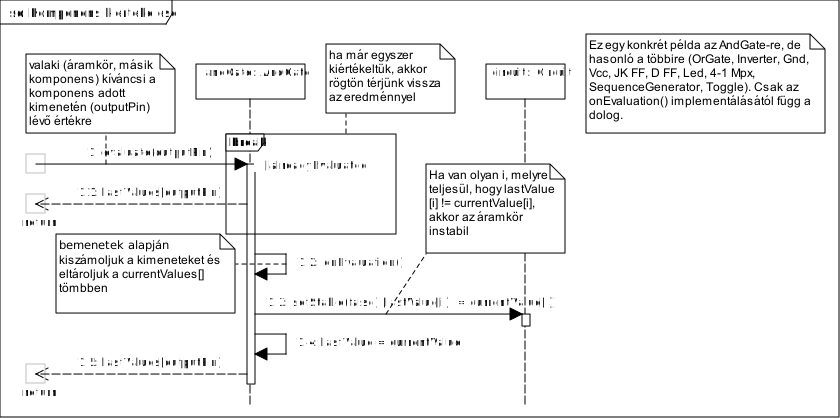
\includegraphics[angle = 90]{chapters/chapter03/seqdiagrams/sim_evaluate.pdf}
\caption{Komponens kiértékelése}
\label{fig:sim_evaluate}
\end{center}
\end{figure}

\begin{figure}[H]
\begin{center}
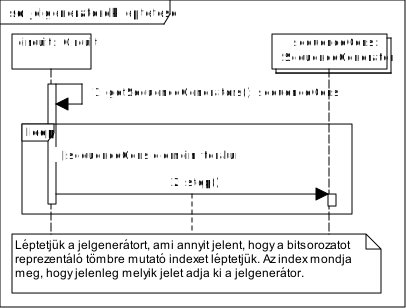
\includegraphics{chapters/chapter03/seqdiagrams/sim_stepGenerators.pdf}
\caption{Jelgenerátorok léptetése}
\label{fig:sim_stepGenerators}
\end{center}
\end{figure}

\begin{figure}[H]
\begin{center}
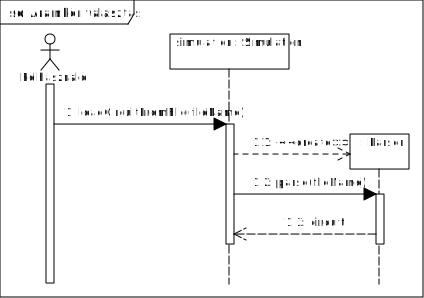
\includegraphics{chapters/chapter03/seqdiagrams/aramkor_valasztas.pdf}
\caption{Áramkör választás}
\label{fig:aramkor_valasztas}
\end{center}
\end{figure}

\begin{figure}[H]
\begin{center}
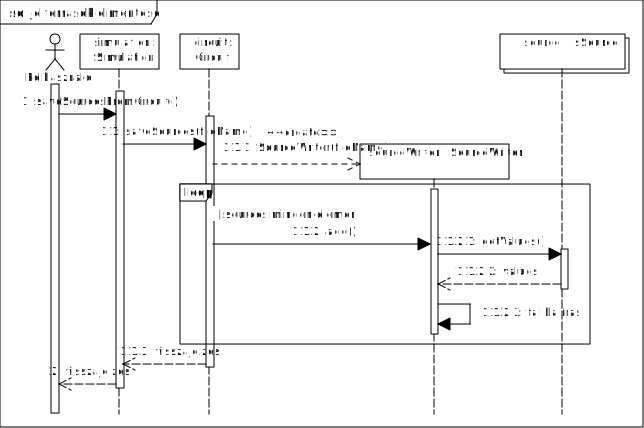
\includegraphics{chapters/chapter03/seqdiagrams/jelforrasok_mentese.pdf}
\caption{Jelforrások mentése}
\label{fig:jelforrasok_mentese}
\end{center}
\end{figure}

\section{State-chartok}
\comment{Csak azokhoz az osztályokhoz, ahol van értelme. Egyetlen állapotból álló state-chartok ne szerepeljenek. A játék működését bemutató state-chart-ot készíteni tilos.}

\begin{figure}[h]
\begin{center}
%\includegraphics[width=17cm]{chapters/chapter03/example.pdf}
\caption{x}
\label{fig:example3}
\end{center}
\end{figure}

